\documentclass{../template/tp}
\usepackage[utf8x]{inputenc}

\usepackage[frenchb]{babel}
\usepackage[T1]{fontenc}

\usepackage{graphicx}
\usepackage{amssymb}
\usepackage{amsmath}
\usepackage{wasysym} %smiley
\usepackage{hyperref}% hyperliens
\usepackage{tikz}
\usetikzlibrary{babel,positioning,calc}
\usepackage[]{circuitikz}
\usepackage{textcomp}
% \usepackage{minted}
\usepackage[long]{datetime}
\usepackage{gensymb} % \ohm, celsius
\usepackage{framed}
\usepackage{pdfpages}
\usepackage{todonotes}
\usepackage{enumitem}
\usepackage{ marvosym }
\usepackage{qrcode}%Don't forget to escape the "#", as the href package requires.

\usepackage{mathastext} % math as standfard text : units are respecting typography conventions.
\usepackage{fancyhdr}
% \langexam{frenchb}

\newboolean{koriG}
\ifx\koriG\undefined
\correction{false}
\else
\correction{true}
\fi

% \correction{false}
% \correction{true}

\author{The Fantastic Four}

%% fancy header & foot
\pagestyle{fancy}
\lhead{[ELEC-H-301] Électronique appliquée\\ TP \no 2 : amplification\ifthenelse{\boolean{corrige}}{~-- Corrigé}{}}
\rhead{v1.0.1\\ page \thepage}
\cfoot{}
%%

\pdfinfo{
/Author (Quentin Delhaye, ULB -- BEAMS)
/Title (TP 2 ELEC-H-301, amplification)
/ModDate (D:\pdfdate)
}

\hypersetup{
pdftitle={TP 2 [ELEC-H-301] Électronique appliquée : Amplification},
pdfauthor={Quentin Delhaye, ©2016 ULB - BEAMS  },
pdfsubject={amplification}
}


\setlength{\parskip}{0.5cm plus4mm minus3mm} %espacement entre §
\setlength{\parindent}{0pt}


\begin{document}

\tptitle{}{Séance 2~: Amplification}

\vspace{-1cm}
%Cette séance d'exercices a pour objectifs de vous apprendre à :
Objectifs : à la fin de cette séance, l'étudiant sera capable de :
\begin{itemize}
\item Déterminer le gain d'un circuit
\item Résoudre un circuit à base d'amplificateur opérationnel à l'aide du zéro virtuel
\item Identifier et caractériser les montages inverseur et non-inverseur
\end{itemize}
\rule{\linewidth}{.5pt}

\Question{%Storey 5th, 15.14

	Quel est le gain en tension du diviseur résistif suivant~?
	\begin{center}
		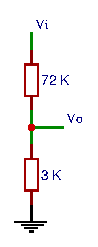
\includegraphics[scale=1.4]{voltage-divider.pdf}
	\end{center}
	% \vspace*{-2cm}
	% \marginpar{\qrcode[hyperlink,height=0.5in]{https://easyeda.com/editor\#id=8OMBL5HoG}}
	% \vspace*{2cm}
	
}
{Nous avons un diviseur résistif, donc $V_{out} = \frac{3 k\Omega}{72 k\Omega + 3 k\Omega} \cdot V_{in}$.
Le gain étant le rapport entre les tensions de sortie et d'entrée, on a un gain $G = \frac{V_{out}}{V_{in}} = 0.04$.}

\Question{%Storey 5th, 14.8

	Un amplificateur a un gain en tension en boucle ouverte de 20, une résistance d'entrée de 10~k\ohm~et une résistance de sortie de 75~\ohm.
	L'entrée de l'amplificateur est connectée à une source de tension de 0.5~V ayant une résistance de sortie de 200~\ohm, et sa sortie est connectée à une résistance de charge de 1~k\ohm.
	Quelle sera la valeur de la tension en sortie~?
	Quel constat pouvez-vous faire au sujet du gain du montage~?
	% \vspace*{-1.5cm}
	% \marginpar{\qrcode[hyperlink,height=0.5in]{https://www.youtube.com/watch?v=dQw4w9WgXcQ}}
	% \vspace*{1.5cm}
}%
{
	\begin{center}
		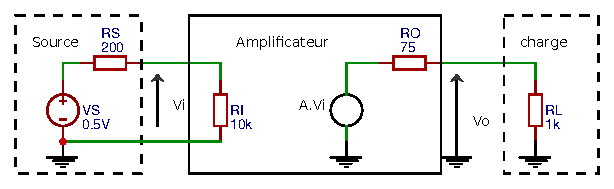
\includegraphics[scale=1.4]{ampli-correction}
	\end{center}

	Commençons par calculer $V_i$.

	\begin{align*}
		V_i & = \frac{R_i}{R_s + R_i} \cdot V_s \\
		& = \frac{10 k\Omega}{200 \Omega + 10 k\Omega} \cdot 0.5 V \\
		& = 0.49 V
	\end{align*}

	Maintenant qu'on sait ce qu'on amplifie, on peut passer à la sortie.

	\begin{align*}
		V_o & = A \cdot V_i \cdot \frac{R_L}{R_o + R_L} \\
		& = 20 \cdot 0.49 \cdot \frac{1 k\Omega}{75 \Omega + 1 k\Omega} \\
		& = 9.12 V
	\end{align*}

	On remarque que le gain du montage est plus faible que 20 à cause des impédances d'entrée et de sortie de l'amplificateur.
	Avec une impédance d'entrée infinie et une de sortie nulle, on aura bien retrouvé ce gain idéal.

}

\Question{%Storey 5th, 16.4

	Présentez les caractéristiques d'un amplificateur opérationnel «~idéal~».
}
{
	\begin{itemize}
		\item Gain infini
		\item Résistance d'entrée infinie
		\item Résistance de sortie nulle
	\end{itemize}
}

\Question{%Storey 5th, 16.5

	Tracez le quadripôle équivalent d'un amplificateur opérationnel idéal.%Je précise « quadripôle » pour leur faciliter la tâche.
}
{
	\begin{center}
		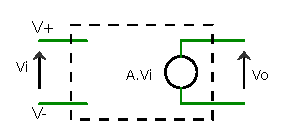
\includegraphics[scale=1.4]{schema-ampli-op.pdf}
	\end{center}
}

\Question{%Storey 5th, 16.18

	Quelles sont les plages usuelles du gain en tension en circuit ouvert et des résistances d'entrée et de sortie d'un amplificateur opérationnel ordinaire~?
}
{
	La plupart des amplificateurs opérationnels ont un gain compris entre 100 et 140 dB (c'est-à-dire entre $10^5$ et $10^7$).
	Les amplis-op FET peuvent avoir une résistance d'entrée allant jusqu'à $10^{12}\Omega$ (alors qu'un bipolaire varie de quelques centaines de kiloohms à une centaine de mégohms).
	Quant à la résistance de sortie, elle varie entre quelques dizaines d'ohms et quelques centaines de kiloohms.
}

\Question{%Storey 5th, 16.19

	Quelles sont les plages usuelles d'alimentation d'un amplificateur opérationnel ordinaire~?
}
{
	Les amplis-op que vous utiliserez en laboratoire seront alimentés en majorité en $\pm 12 V$.
	Certains peuvent cependant être alimentés jusqu'en $\pm 30 V$, ou jusqu'aussi bas que $\pm 1.5 V$.

	Il est aussi courant d'alimenter un ampli-op de façon asymétrique en connectant une des deux bornes à la masse.
	Ce cas sera étudié dans la séance d'exercices \no 3.
}

\Question{%Storey 5th, 14.23

	Un amplificateur différentiel a un gain en tension de 100.
	Si une tension de 18.3~V est appliquée à son entrée non-inverseuse et qu'une tension de 18.2~V est appliquée à son entrée inverseuse, quelle est la tension de sortie~?
}
{
	La tension d'entrée d'un amplificateur différentiel vaut $V_+ - V_-$ (respectivement l'entrée non-inverseuse et inverseuse), c'est-à-dire 0.1~V dans notre cas.
	La tension de sortie vaudra donc $(V_+ - V_-) \cdot 100 = 10 V$.
}

\Question{%Ex labo 2, 1.1

	Soit le montage ci-dessous, comprenant un ampli-op de gain $10^5$.

	\begin{center}
		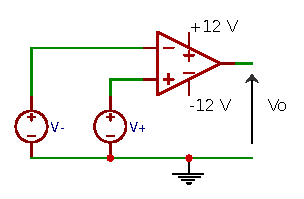
\includegraphics[scale=1.4]{multi-source}
	\end{center}
	% \vspace*{-2cm}
	% \marginpar{\qrcode[hyperlink,height=0.5in]{https://easyeda.com/editor\#id=lQMT0JA4h}}
	% \vspace*{2cm}

	Que vaut $V_{out}$ dans les cas suivants~:
	\begin{center}
		\begin{tabular}{c|c}
		$V_+$ & $V_-$ \\ \hline
		1 $\mu$V & 0 V \\
		0 V & 1 V \\
		0 V & 1 V $\cdot \sin(2 \cdot \pi \cdot 1000 \cdot t)$ \\
		1 V $\cdot \sin(2 \cdot \pi \cdot 1000 \cdot t)$ & -3 V \\
		1 $\mu$V $\cdot \sin(2 \cdot \pi \cdot 1000 \cdot t)$ & -3 V \\
		1 $\mu$V $\cdot \sin(2 \cdot \pi \cdot 1000 \cdot t)$ & 0 V \\
		\end{tabular}
	\end{center}
}
{
	\begin{enumerate}[label=\alph*)]
		\item $V_+$ = 1 $\mu$V et $V_-$ = 0 V

			$V_{out} = A \cdot (V_+ - V_-) = 100 mV$

		\item $V_+$ = 0 V et $V_-$ = 1 V

			$V_{out} = -12 V$

			Par calcul, la tension de sortie devrait valoir -100000~V, mais elle sature sur la tension d'alimentation.

		\item $V_+$ = 0 V et $V_-$ = 1 V $\cdot \sin(2 \cdot \pi \cdot 1000 \cdot t)$

			La sortie sature à nouveau sur les bornes d'alimentation. On obtient en sortie une onde carrée d'amplitude $\pm$12~V, d'un rapport cyclique de 50~\% et d'une période de 1~ms. Autrement dit, les $0.5 \cdot 10^{-3}$ premières secondes de la période, le signal est à 12~V et les $0.5 \cdot 10^{-3}$ suivantes à -12~V. Lorsque la sortie ne sature pas ($-12<V_{out}<12$), $V_{out}=A\cdot\left(V+-V-\right)$

		\item $V_+$ = 1 V $\cdot \sin(2 \cdot \pi \cdot 1000 \cdot t)$ et $V_-$ = -3 V

			$V_{out} = 12 V$

			En effet, le minimum de la tension d'entrée étant 2~V, une fois amplifié, le signal sature sur l'alimentation.

		\item $V_+$ = 1 $\mu$V $\cdot \sin(2 \cdot \pi \cdot 1000 \cdot t)$ et $V_-$ = -3 V

			$V_{out} = 12 V$

		\item $V_+$ = 1 $\mu$V $\cdot \sin(2 \cdot \pi \cdot 1000 \cdot t)$ et $V_-$ = 0 V

			$V_{out} = 100 mV \cdot \sin(2 \cdot \pi \cdot 1000 \cdot t)$
	\end{enumerate}
}

\Question{

	Expliquez le principe du zéro virtuel et ses conditions d'application.
}
{
	On peut définir le principe comme suit~: «~Tant qu'un amplificateur opérationnel ne sature pas, sa tension différentielle  d'entrée est virtuellement nulle.~»

	On considère donc à la fois que $V^+ = V^-$ et que le gain de l'ampli-op (pas celui du montage) est infini.

	Ce principe n'est cependant applicable que lorsque l'ampli-op ne sature pas.
}

\Question{%Ex labo 2, 1.2

	Résolvez les circuits suivants en utilisant le principe du zéro virtuel, avec $R_1 = 1 k\ohm$ et $R_2 = 10 k\ohm$~:

	\begin{minipage}{0.5\linewidth}
		\begin{center}
			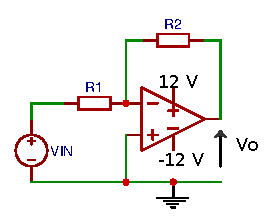
\includegraphics[scale=1.4]{inverseur.pdf}
		\end{center}
	\end{minipage}
	\begin{minipage}{0.45\linewidth}
		\begin{center}
			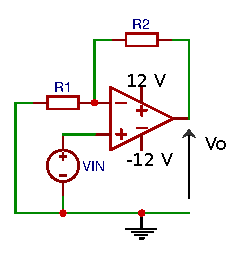
\includegraphics[scale=1.4]{non-inverseur.pdf}
		\end{center}
	\end{minipage}
	% \vspace*{-4cm}
	% \marginpar{\qrcode[hyperlink,height=0.5in]{https://easyeda.com/editor\#id=fgnFPDLBb}}
	% \vspace*{4cm}
	% \vspace*{-2cm}
	% \marginpar{\qrcode[hyperlink,height=0.5in]{https://easyeda.com/editor\#id=Q2wKSCmvL}}
	% \vspace*{2cm}

	\begin{enumerate}[label=\alph*)]
		\item Pour $V_{in} = 500 mV \cdot \sin(2\cdot \pi \cdot 1000 \cdot t)$
		\item Pour $V_{in} = -4V$
		\item Pour $V_{in} = 4V \cdot \sin(2\cdot \pi \cdot 1000 \cdot t)$
	\end{enumerate}
}
{
	\begin{enumerate}
		\item Étant donné que $V_+ = V_-$, on a $V_- = 0 V$. En appliquant la loi d'Ohm, on peut trouver le courant circulant dans $R_1$ : $i_1 = \frac{V_{in}}{R_1}$. L'entrée de l'ampli-op ayant une impédance infinie, le courant entrant dans l'ampli-op est nul. On a donc $i_1 = i_2$. Via la maille partant de la masse à l'entrée non-inverseuse, à la masse de la tension de sortie, on a $V_{o} = -R_2\cdot i_2 = -\frac{R_2}{R_1}\cdot V_{in}$.
		\begin{enumerate}[label=\alph*)]
			\item Pour $V_{in} = 500 mV \cdot \sin(2\cdot \pi \cdot 1000 \cdot t)$

			$V_o = -5V \cdot \sin(2\cdot \pi \cdot 1000 \cdot t)$

			\item Pour $V_{in} = -4V$

			$V_o = 12 V$

			\item Pour $V_{in} = 4V \cdot \sin(2\cdot \pi \cdot 1000 \cdot t)$

			$V_o = -40 V \cdot \sin(2\cdot \pi \cdot 1000 \cdot t)$ avec saturation à $\pm$12~V.
			
		\end{enumerate}
		\item  Par le zéro virtuel, $V_+ = V_- = V_{in}$.
		Par la loi d'Ohm et la maille partant de la masse connectée à la résistance $R_1$ jusqu'à la masse de la source de tension, on trouve $i_1 = \frac{V_{in}}{R_1}$.
		L'entrée de l'ampli-op ayant une impédance infinie, le courant entrant dans l'ampli-op est nul. On a donc $i_1 = i_2$.
		En appliquant la loi d'Ohm à la maille partant de la masse connectée à $R_1$ jusqu'à la masse de la tension de sortie, on peut trouver $V_o = V_{in} + R_2\cdot i_2 = V_{in} + R_2 \cdot \frac{V{in}}{R_1} = (1 + \frac{R_2}{R_1}) \cdot V_{in}$.
		\begin{enumerate}[label=\alph*)]
			\item Pour $V_{in} = 500 mV \cdot \sin(2\cdot \pi \cdot 1000 \cdot t)$

			$V_o = 5.5 V \cdot \sin(2\cdot \pi \cdot 1000 \cdot t)$

			\item Pour $V_{in} = -4V$

			$V_o = -12 V$

			\item Pour $V_{in} = 4V \cdot \sin(2\cdot \pi \cdot 1000 \cdot t)$

			$V_o = 44 V \cdot \sin(2\cdot \pi \cdot 1000 \cdot t)$ avec saturation à $\pm$12~V.
			
		\end{enumerate}
	\end{enumerate}
}

\Question{%Storey 5th, 15.16, ampli non-inverseur

	Déterminez le gain en tension du montage amplificateur suivant~:
	\begin{center}
		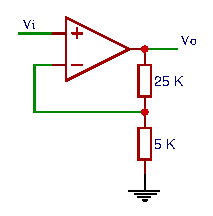
\includegraphics[scale=1.4]{non-inverseur-storey-15-16}
	\end{center}
	% \vspace*{-2cm}
	% \marginpar{\qrcode[hyperlink,height=0.5in]{https://easyeda.com/editor\#id=dvL4aBM6E}}
	% \vspace*{2cm}
}
{
	Gain du montage non-inverseur~: $ 1 + \frac{25 k\Omega}{5 k\Omega} = 6$.
}

\Question{%Ex labo 2, 2.2

	Résolvez le circuit suivant~:
	\begin{center}
		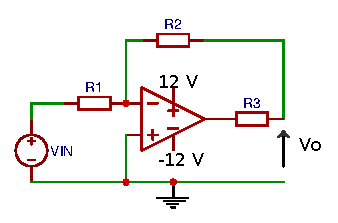
\includegraphics[scale=1.4]{inverseur-charge}
	\end{center}
	% \vspace*{-2cm}
	% \marginpar{\qrcode[hyperlink,height=0.5in]{https://easyeda.com/editor\#id=Z0SE3MLTt}}
	% \vspace*{2cm}


	\begin{enumerate}[label=\alph*)]
		\item Avec $R_1 = 1 k\ohm$, $R_2 = 10 k\ohm$, $R3 = 1 k\ohm$ et $V_{in} = 2 V \cdot sin(2 \cdot \pi \cdot 1000 \cdot t)$
		\item Avec $R_1 = 1 k\ohm$, $R_2 = 10 k\ohm$, $R3 = 20 k\ohm$ et $V_{in} = 2 V \cdot sin(2 \cdot \pi \cdot 1000 \cdot t)$
	\end{enumerate}
}
{
	En résolvant le circuit à l'aide du zéro virtuel, il apparaît que la résistance n'a aucune influence sur le gain.
	On trouve donc $V_{o} = - \frac{R_2}{R_1} \cdot V_{in}$.

	Cependant, le principe du zéro virtuel n'est valable que lorsque l'ampli-op ne sature pas.
	Lorsque ce dernier sature sur son alimentation positive (de 12~V dans notre cas), le circuit devient le suivant~:
	\begin{center}
		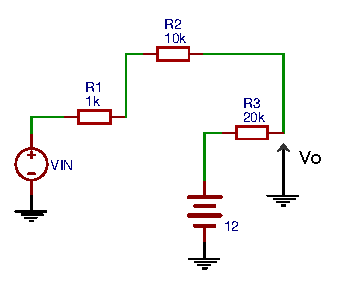
\includegraphics[scale=1.4]{inverseur-charge-saturation.pdf}
	\end{center}

	En considérant la maille complète, on peut trouver le courant y circulant :
	\begin{align*}
	V_{in} & = i \cdot R_1 + i \cdot R_2 + i \cdot R_3 + 12\\
	\Leftrightarrow i & = \frac{V_{in} - 12}{R_1 + R_2 + R_ 3}
	\end{align*}

	En ne prenant que la maille entre la source d'alimentation continue et la sortie $V_o$, on trouve~:
	\begin{align*}
	V_o & = 12 + i \cdot R_3 \\
	& = 12 + (V_{in} - 12) \cdot \frac{R_3}{R_1 + R_2 + R_ 3}
	\end{align*}

	Pour $R_3 = 20 k\Omega$, on obtient le résultat suivant~:

	\begin{center}
		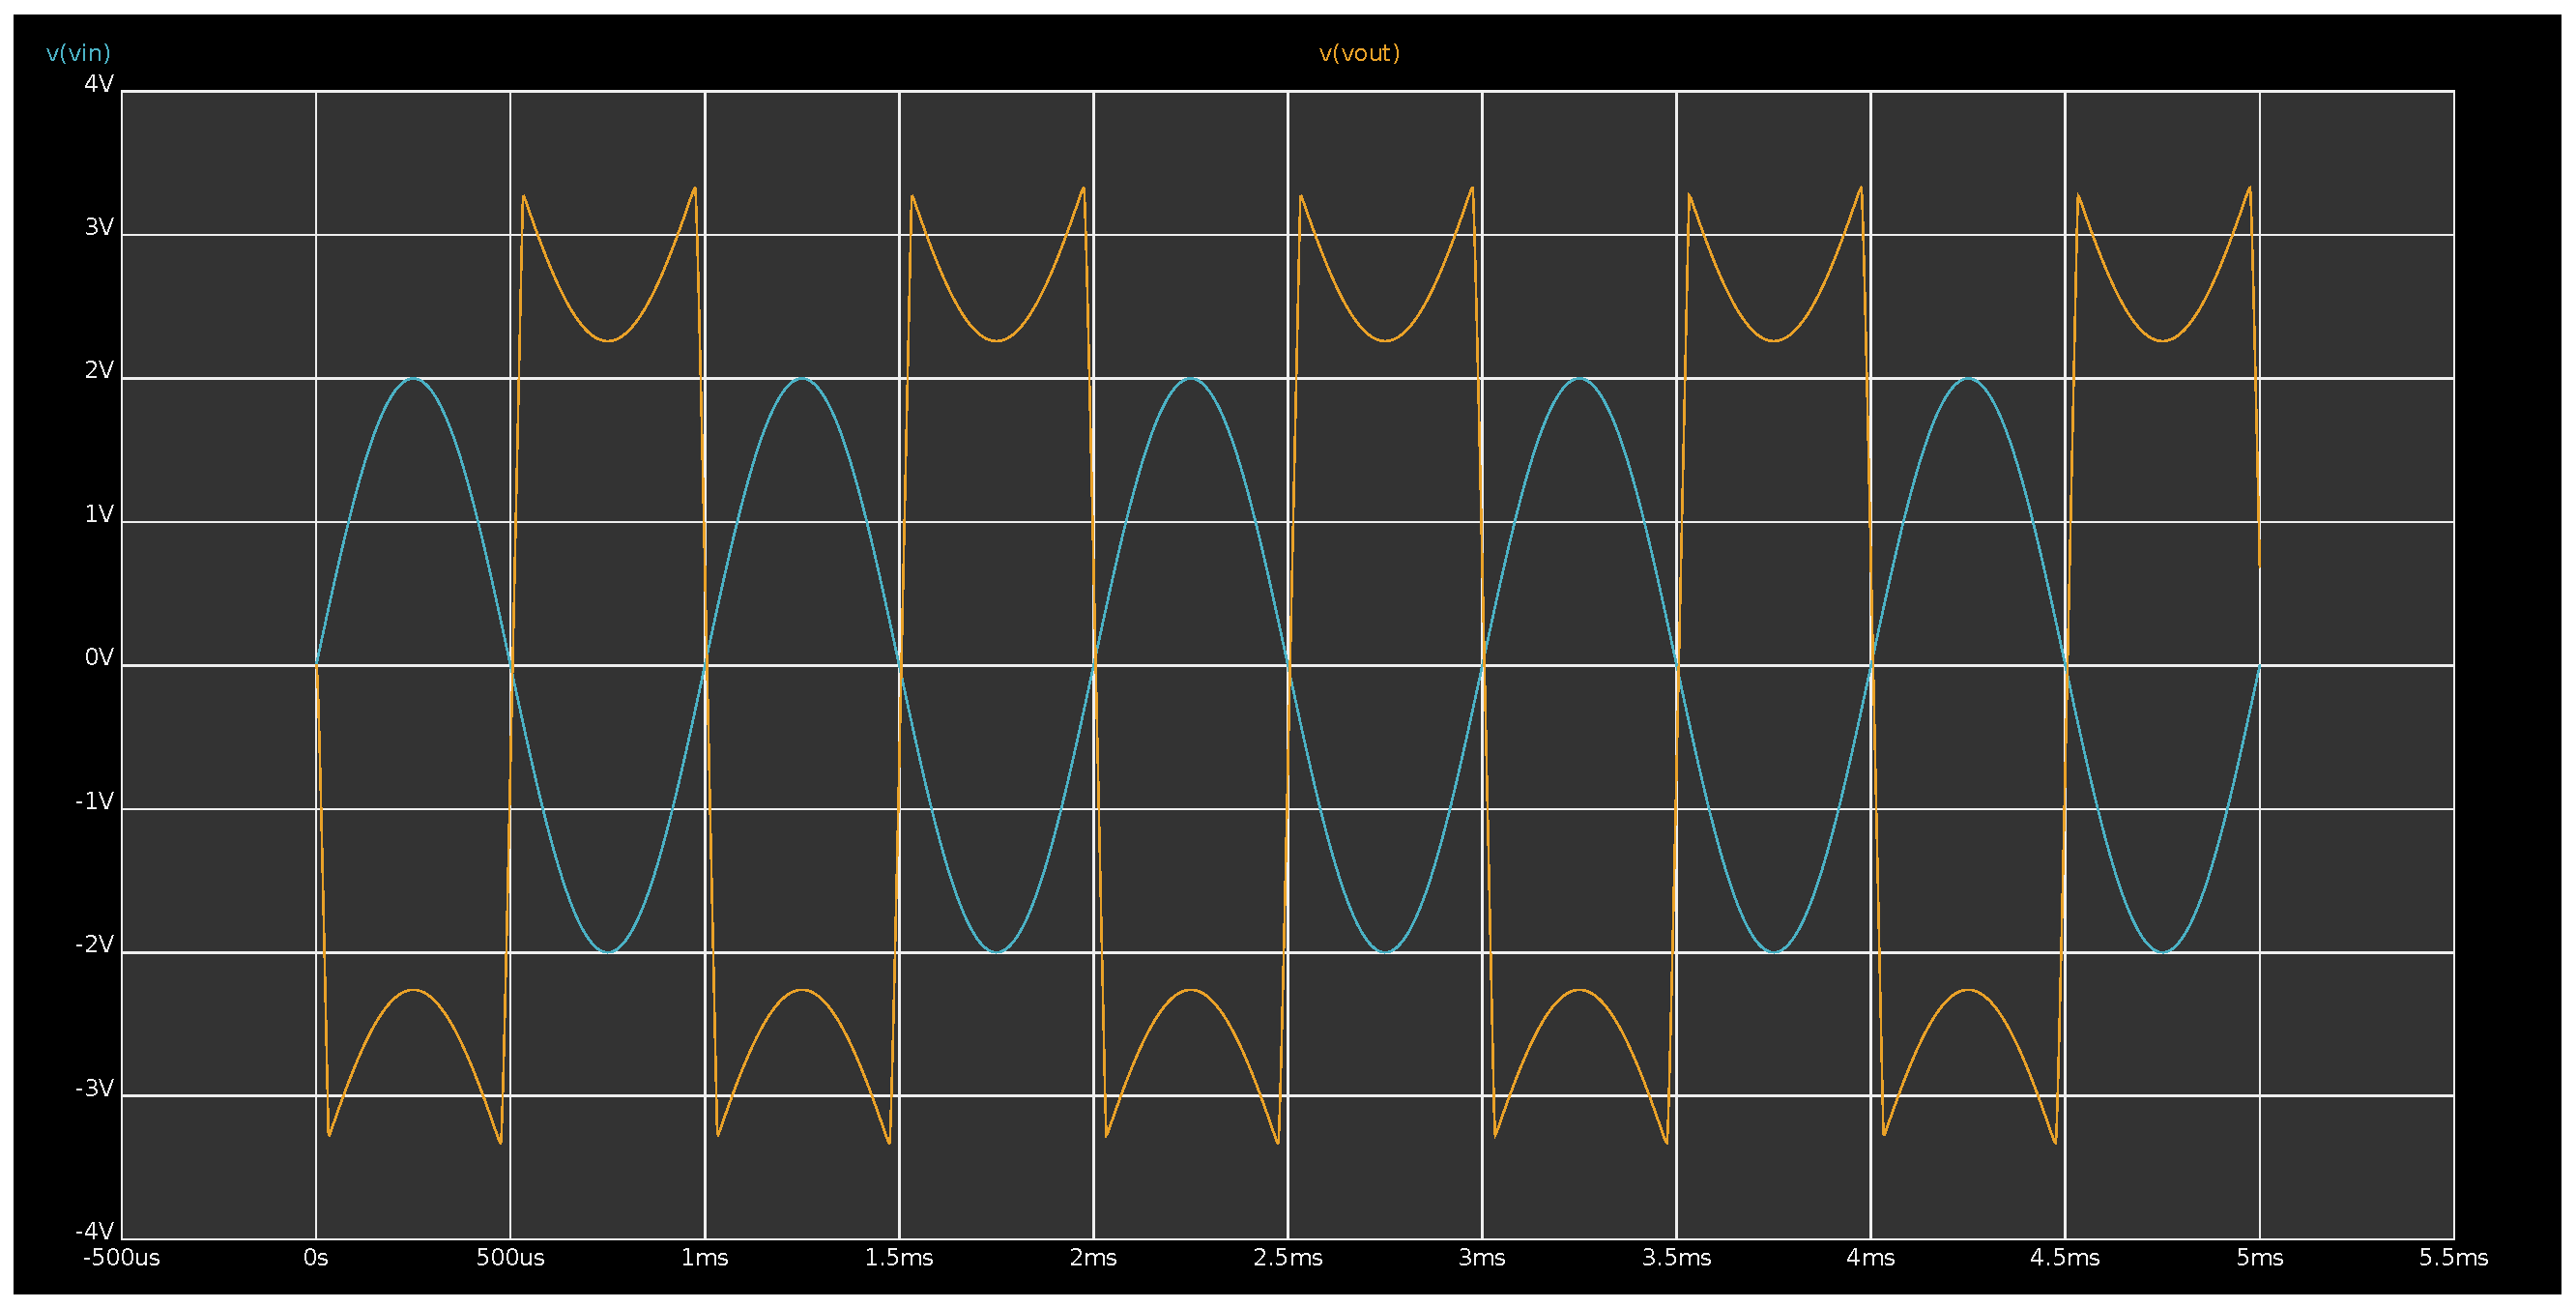
\includegraphics[width=\textwidth]{inverseur-charge-saturation-waveform.pdf}
	\end{center}
}

\Question{%Ex labo 2, 2.1

	Résolvez le circuit suivant~:

	\begin{center}
		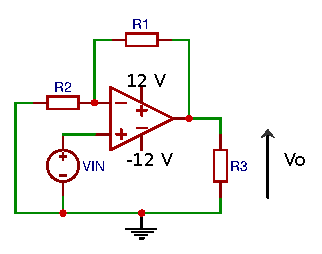
\includegraphics[scale=1.4]{non-inverseur-charge}
	\end{center}
	% \vspace*{-2cm}
	% \marginpar{\qrcode[hyperlink,height=0.5in]{https://easyeda.com/editor\#id=rS5UEofWa}}
	% \vspace*{2cm}

	Avec $R_1 = 1 k\ohm$, $R_2 = 5 k\ohm$, $R_3 = 1 k\ohm$ et $V_{in} = 500 mV \cdot sin(2 \cdot \pi \cdot 1000 \cdot t)$
}
{
	En utilisant le principe du zéro virtuel, on trouve que $R_3$ n'a aucune influence sur le gain du montage (et la tension de sortie en particulier)~: $V_o = (1+ \frac{R_1}{R_2}) \cdot V_{in}$.

	L'influence de $R_3$ s'applique sur l'intensité du courant sortant de l'ampli-op~: $i_3 = \frac{V_o}{R_3}$.
}

\Question{%Ex labo 2, 2.3

	Soit les montages suivants~:

	\begin{minipage}{0.5\linewidth}
		\begin{center}
			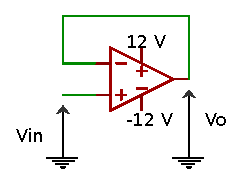
\includegraphics[scale=1.4]{suiveur-pur.pdf}
		\end{center}
	\end{minipage}
	\begin{minipage}{0.45\linewidth}
		\begin{center}
			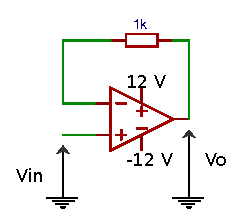
\includegraphics[scale=1.4]{suiveur-retroaction.pdf}
		\end{center}
	\end{minipage}
	% \vspace*{-4cm}
	% \marginpar{\qrcode[hyperlink,height=0.5in]{https://easyeda.com/editor\#id=31d6FpQne}}
	% \vspace*{4cm}
	% \vspace*{-2cm}
	% \marginpar{\qrcode[hyperlink,height=0.5in]{https://easyeda.com/editor\#id=ME1lkDiHD}}
	% \vspace*{2cm}

	\begin{enumerate}
		\item Calculez le gain en tension.
		\item Quelle est l'utilité de ce genre de montage~?
		\item Pour illuster votre réponse, on souhaite connecter les deux blocs suivants~:
		\begin{center}
			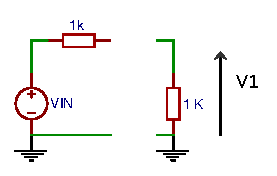
\includegraphics[scale=1.4]{montage-pour-suiveur.pdf}
		\end{center}
		% \vspace*{-2cm}
		% \marginpar{\qrcode[hyperlink,height=0.5in]{https://easyeda.com/editor\#id=TrtMXgD0G}}
		% \vspace*{2cm}

		Calculez $V_1$~:
		\begin{itemize}
			\item en connectant directement les deux blocs~;
			\item en insérant un des deux montages ci-dessus entre les deux blocs.
		\end{itemize}
	\end{enumerate}
}
{
	\begin{enumerate}
		\item Calculez le gain en tension.
		\begin{enumerate}[label=\alph*)]
			\item Par le principe du zéro virtuel, on a $V_{in} = V_+ = V_- = V_o$, le gain vaut donc 1.
			\item Avec le sempiternel zéro virtuel, on a $V_{in} = V_+ = V_-$. Puisque la résistance d'entrée de l'ampli-op est infinie, le courant circulant dans la branche de rétroaction est nul. Il n'y a donc pas de chute de tension dans la résistance et $V_o = V_- = V_{in}$. Le gain vaut aussi 1.
		\end{enumerate}

		\item Ce genre de montage, qu'on appelle « suiveur », sert à l'adaptation d'impédance.

		\item Illustrons son utilité.
		\begin{itemize}
			\item En connectant directemet les deux blocs, on obtient un simple diviseur résistif~: $V_1 = \frac{1k\Omega}{1k\Omega+1k\Omega} \cdot V_{in} = \frac{1}{2}\cdot V_{in}$, ce qui donne un gain de $0.5$.

			\item En insérant un suiveur entre les deux blocs, on crée le montage suivant~:
			\begin{center}
				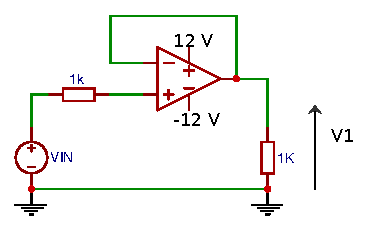
\includegraphics[scale=1.4]{suiveur-adaptation-impedance.pdf}
			\end{center}

			Le gain du montage est toujours de 1 et on retrouve bien la tension d'entrée à la sortie.
		\end{itemize}
		\item %Ajout d'une résistance dans la boucle de rétroaction\\
		L'ajout d'une résistance dans la boucle de rétroaction permet d'équilibrer les courants de polarisation des entrées $+$ et $-$ de l'ampli, en supposant que l'impédance de sortie de la source soit du même ordre de grandeur. Ceci permet d'améliorer les performances de l'amplificateur en diminuant l'influence du courant de polarisation sur la tension de sortie mais aussi de simplifier la réalisation du circuit. Ces considérations dépassent le cadre de ce cours.
	\end{enumerate}
}

\Question{\label{q.res-serie}%Ex labo 2, 2.4

	Résolvez les montages suivants~:

	\begin{enumerate}
		\item $R_1 = 1 k\ohm$, $R_2 = 5 k\ohm$, $R_3 = 1 k\ohm$ and $V_{in} = 500 mV \cdot sin(2 \cdot \pi \cdot 1000 \cdot t)$

		\begin{center}
			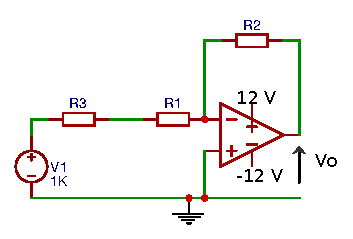
\includegraphics[scale=1.4]{inverseur-entree-serie.pdf}
		\end{center}
		% \vspace*{-2cm}
		% \marginpar{\qrcode[hyperlink,height=0.5in]{https://easyeda.com/editor\#id=UxggzF8uD}}
		% \vspace*{2cm}

		\item $R_1 = 1 k\ohm$, $R_2 = 5 k\ohm$, $R_3 = 1 k\ohm$, $R_4 = 1k\Omega$, $R_5 = 500\Omega$ et $V_{in} = 500 mV \cdot sin(2 \cdot \pi \cdot 1000 \cdot t)$

		\begin{center}
			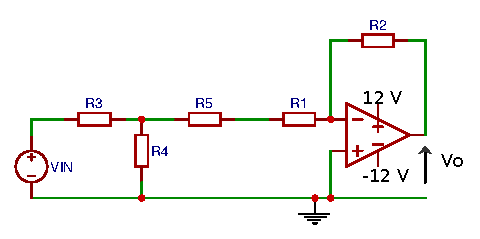
\includegraphics[scale=1.4]{inverseur-resistances-en-folie.pdf}
		\end{center}
		% \vspace*{-2cm}
		% \marginpar{\qrcode[hyperlink,height=0.5in]{https://easyeda.com/editor\#id=oOdkyvbeM}}
		% \vspace*{2cm}
	\end{enumerate}
}
{
	\begin{enumerate}
		\item On peut fusionner $R_1$ et $R_3$ qui sont en série, mettant en évidence un simple montage inverseur~: $V_o = - \frac{R_2}{R_1 + R_3} \cdot V_1 = - 1.25 V \cdot \sin(2\cdot \pi \cdot 1000 t)$.

		\item Il faut procéder en deux étapes~:
		\begin{itemize}
			\item Les résistances $R_1$ et $R_5$ sont en série et peuvent être englobées dans une résistance $R_s = R_1 + R_5$.
			\item Le dipôle constitué par $V_{in}$, $R_3$ et $R_4$ peut être remplacé par son équivalent de Thévenin~:
			\begin{itemize}
				\item $V_{eq} = V_{in} \cdot \frac{R_4}{R_3 + R_4} = 250 mV \cdot \sin(2\cdot \pi \cdot 1000 t)$
				\item $R_{eq} = R_3 // R_4 = \frac{R_3 \cdot R_4}{R_3 + R_4} = 500 \Omega$
			\end{itemize}

		On a ainsi $V_o = -\frac{R_2}{R_s + R_{eq}} \cdot V_{eq} = - 625 mV \cdot \sin(2\cdot \pi \cdot 1000 t)$
		\item [2'] Il est aussi de calculer directement l'équivalent de Thévenin de $\left\lbrace V_{IN}, R1, R3, R4, R5 \right\rbrace$.
		\end{itemize}
	\end{enumerate}

}

\Question{%Storey 5th, 16.14, superposition

	Déterminez l'expression de la tension de sortie $V_o$ des circuits suivants en fonction des entrées $V_1$ et $V_2$.
	Déduisez-en la valeur de la tension de sortie si $V_1 = 1 V$ et $V_2 = 0.5 V$.

	\begin{minipage}{0.5\linewidth}
		\begin{center}
			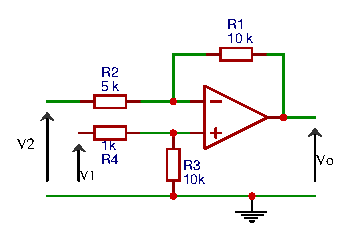
\includegraphics[scale=1.4]{storey-16-14.pdf}
		\end{center}
	\end{minipage}
	\begin{minipage}{0.45\linewidth}
		\begin{center}
			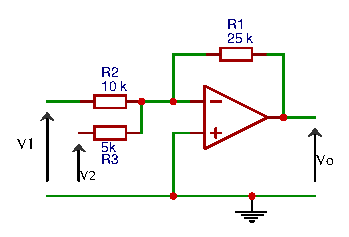
\includegraphics[scale=1.4]{storey-16-15.pdf}
		\end{center}
	\end{minipage}
	% \vspace*{-4cm}
	% \marginpar{\qrcode[hyperlink,height=0.5in]{https://easyeda.com/editor\#id=XIM1U0HNJ}}
	% \vspace*{4cm}
	% \vspace*{-2cm}
	% \marginpar{\qrcode[hyperlink,height=0.5in]{https://easyeda.com/editor\#id=lsYCysvF8}}
	% \vspace*{2cm}
}
{
	% Je n'aime pas du tout la résolution de Storey, il fait tout d'un coup comme un bourrin. Je préfère le faire par superposition.
	\begin{enumerate}[label=\alph*)]
		\item Le système étant linéaire, nous allons procéder par superposition en nous occupant de $V_1$ et $V_2$ séparément.
		\begin{itemize}
			\item Considérons d'abord uniquement $V_1$ et en remplaçant $V_2$ par un court-circuit.
			On peut remplacer le groupe $V_1$, $R_3$ et $R_4$ par son équivalent de Thévenin~: $V_{th} = \frac{R_3}{R_3 + R_4} \cdot V_1$.
			Il n'est pas nécessaire de s'intéresser à la résistance équivalent de Thévenin car elle n'occasionnera aucune chute de tension étant donné qu'aucun courant ne rentre dana l'ampli-op.
			On a donc un simple montage non-inverseur, ce qui donne $V_o = (1+\frac{R_1}{R_2}) \cdot V_{th}$.

			\item Considérons à présent la réciproque en remplaçant $V_1$ par un court-circuit.
			Les résistances à l'entrée non-inverseuse peuvent à nouveau être ignorées, ce qui nous donne un montage inverseur classique :
			$V_o = -\frac{R_1}{R_2} \cdot V_2$
		\end{itemize}

		Il ne nous reste plus qu'à superposer les deux solutions en les additionnant~:
		\begin{align*}
		V_o & = (1+\frac{R_1}{R_2}) \cdot V_{th} - \frac{R_1}{R_2} \cdot V_2 \\
		& = (1+\frac{R_1}{R_2}) \cdot \frac{R_3}{R_3 + R_4} \cdot V_1 - \frac{R_1}{R_2} \cdot V_2 \\
		& = (1+\frac{10k}{5k}) \cdot \frac{10k}{10k + 1k} \cdot V_1 - \frac{10k}{5k} \cdot V_2 \\
		& = 2.73 \cdot V_1 - 2 \cdot V_2 \\
		& = 1.73 V
		\end{align*}

		\item En utilisant le théorème de superposition, on peut séparer le montage en deux sous-montages inverseurs en remplaçant alternativement $V_1$ puis $V_2$ par un court-circuit.
		On trouve alors 
		\begin{align*}
		V_o & = -\frac{R_1}{R_2} \cdot V_1 - \frac{R_1}{R_3} \cdot V_2 \\
		& = - 2.5 \cdot V_1 - 5 \cdot V_2 \\
		& = -5V
		\end{align*}
	\end{enumerate}
}

\Question{%Ex labo 2, 2.5

	Résolvez le circuit suivant~:

	\begin{center}
		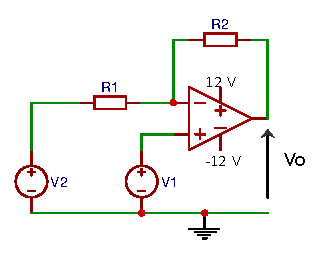
\includegraphics[scale=1.4]{sources-multiples.pdf}
	\end{center}
	% \vspace*{-2cm}
	% \marginpar{\qrcode[hyperlink,height=0.5in]{https://easyeda.com/editor\#id=kF4UCTXpG}}
	% \vspace*{2cm}

	\begin{enumerate}[label=\alph*)]
		\item $R_1 = 1 k\ohm$, $R_2 = 5 k\ohm$, $V_1 = 500 mV \cdot sin(2 \cdot \pi \cdot 1000 \cdot t)$ et $V_2 = 50 mV \cdot sin(2 \cdot \pi \cdot 500 \cdot t)$
		\item $R_1 = 1 k\ohm$, $R_2 = 20 k\ohm$, $V_1 = 100 mV \cdot sin(2 \cdot \pi \cdot 1000 \cdot t)$ et $V_2 = 50 mV \cdot sin(2 \cdot \pi \cdot 1000 \cdot t)$
	\end{enumerate}
}
{
	En utilisant le théorème de superposition, c'est-à-dire en remplaçant alternativement $V_1$ et $V_2$ par un court-circuit, on peut mettre en évidence un sous-montage non-inverseur (avec $V_1$) et un inverseur (avec $V_2$).
	On obtient donc $V_o = (1+\frac{R_2}{R_1}) \cdot V_1 - \frac{R_2}{R_1} \cdot V_2$.

	\begin{enumerate}[label=\alph*)]
		\item $V_o = 3V \cdot sin(2 \cdot \pi \cdot 1000 \cdot t) - 250mV \cdot sin(2 \cdot \pi \cdot 500 \cdot t)$

		\item $V_o = 1.1 V \cdot sin(2 \cdot \pi \cdot 1000 \cdot t)$

		Attention, on ne peut additionner l'amplitude des sinusoïdes que si elles ont la même fréquence et la même phase.
	\end{enumerate}
}

\Question{%Ex labo 2, 2.6

	Résolvez les circuits suivants avec $R_1 = 1 k\ohm$, $R_2 = 5 k\ohm$ , $R_3 = 4 k\ohm$ et $I_1 = 0.5 mA$~:

	\begin{minipage}{0.5\linewidth}
		\begin{center}
			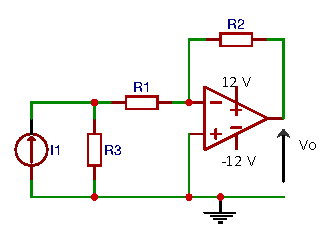
\includegraphics[scale=1.4]{inverseur-source-de-courant.pdf}
		\end{center}
	\end{minipage}
	\begin{minipage}{0.45\linewidth}
		\begin{center}
			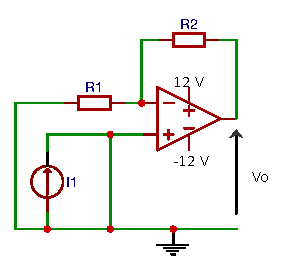
\includegraphics[scale=1.4]{non-inverseur-source-de-courant.pdf}
		\end{center}
	\end{minipage}
	% \vspace*{-4cm}
	% \marginpar{\qrcode[hyperlink,height=0.5in]{https://easyeda.com/editor\#id=GinhOxIUi}}
	% \vspace*{4cm}
	% \vspace*{-2cm}
	% \marginpar{\qrcode[hyperlink,height=0.5in]{https://easyeda.com/editor\#id=NrLCiPeY2}}
	% \vspace*{2cm}
}
{
	\begin{enumerate}
		\item Calculons l'équivalent de Thévenin du couple $I_1$ et $R_3$~: $V_{th} = I_1 \cdot R_3$ et $R_{th} = R_3$.

		On retrouve alors un montage similaire à l'exercice~\ref{q.res-serie}.
		La sortie de ce montage inverseur sera~:
		\begin{align*}
		V_o & = - \frac{R_2}{R_1 + R_{th}} \cdot V_{th} \\
		& = - \frac{R_2}{R_1 + R_3} \cdot I_1 \cdot R_3 \\
		& = -2 V
		\end{align*}

		\item Ce circuit est trivial. Étant donné qu'aucun courant n'entre dans l'ampli-op (résistance d'entrée infinie), la source de courant débite tout son courant dans un court-circuit relié à la masse.
		La tension d'entrée est donc nulle, tout comme celle de sortie.
	\end{enumerate}
}

\Question{Examen de janvier 2005%Ex labo 2, janvier 2005

	\begin{center}
		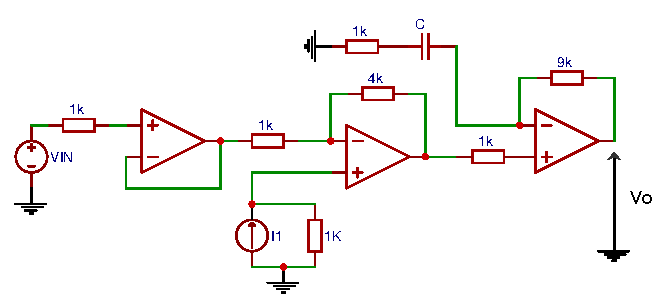
\includegraphics[scale=1.4]{cascade.pdf}
	\end{center}
	% \vspace*{-4cm}
	% \marginpar{\qrcode[hyperlink,height=0.5in]{https://easyeda.com/editor\#id=FjN7mxG21}}
	% \vspace*{4cm}

	On considère le montage ci-dessus pour lequel~:
	\begin{itemize}
		\item $V_{in} = 50 mV \cdot \sin(2\cdot \pi \cdot 50 t)$
		\item $I_1 = 1 \mu A$
		\item À la fréquence de la source de tension, la capacité $C$ peut être considérée comme un court-circuit.
	\end{itemize}

	\begin{enumerate}
		\item Calculez les composantes continue et alternative de la tension $V_{out}$.
		\item Indiquez l'utilité du premier étage à ampli-op.
	\end{enumerate}
}
{
	\begin{enumerate}
		\item Nous allons procéder par étage et par superposition lorsque nécessaire.
		\begin{itemize}
			\item Commençons par le premier étage dont la sortie est prise juste après le premier ampli-op.
			Nous avons un simple suiveur, la sortie reprend la valeur de l'entrée.

			\item Le deuxième étage comprend deux sources que nous allons étudier séparément avant de les superposer.
			\begin{enumerate}[label=\alph*)]
				\item Sortie due à $V_{in}$~: $-4 \cdot V_{in}$ (montage inverseur).
				\item Sortie due à la source de courant~: la source de tension équivalente par Thévenin est $V_{th} = I_1 \cdot 1k = 1 mV$.
				Cette source équivalente passe dans un montage non-inverseur de gain 5, la sortie vaut 5~mV.
			\end{enumerate}

			À la sortie du second étage, on obtient $5 mV - 4 \cdot V_{in}$.

			\item Pour le troisième étage, il convient de séparer l'étude des sources alternatives et continues.
			\begin{enumerate}[label=\alph*)]
				\item La source alternative entre dans un montage non-inverseur de gain 10, la sortie vaut $-40 \cdot V_{in}$ (condensateur = court-circuit).
				\item Pour la source continue, le condensateur se comporte comme un circuit ouvert, elle entre donc dans un autre étage suiveur, la sortie reprend la valeur de l'entrée~: 5~mV.
			\end{enumerate}

			En conséquence, $V_o = 5 mV - 2 V \cdot \sin(2\cdot \pi \cdot 50 t)$
		\end{itemize}

		\item Le premier étage sert à assurer l'adaptation d'impédance (en tension) entre la source alternative et le premier bloc amplificateur.
	\end{enumerate}

}



\end{document}